%%%%%%%%%%%%%%%%%%%%%%% file template.tex %%%%%%%%%%%%%%%%%%%%%%%%%
%
% This is a general template file for the LaTeX package SVJour3
% for Springer journals.          Springer Heidelberg 2010/09/16
%
% Copy it to a new file with a new name and use it as the basis
% for your article. Delete % signs as needed.
%
% This template includes a few options for different layouts and
% content for various journals. Please consult a previous issue of
% your journal as needed.
%
%%%%%%%%%%%%%%%%%%%%%%%%%%%%%%%%%%%%%%%%%%%%%%%%%%%%%%%%%%%%%%%%%%%
%
% First comes an example EPS file -- just ignore it and
% proceed on the \documentclass line
% your LaTeX will extract the file if required
% \begin{filecontents*}{example.eps}
% %!PS-Adobe-3.0 EPSF-3.0
% %%BoundingBox: 19 19 221 221
% %%CreationDate: Mon Sep 29 1997
% %%Creator: programmed by hand (JK)
% %%EndComments
% gsave
% newpath
%   20 20 moveto
%   20 220 lineto
%   220 220 lineto
%   220 20 lineto
% closepath
% 2 setlinewidth
% gsave
%   .4 setgray fill
% grestore
% stroke
% grestore
% \end{filecontents*}
%
\RequirePackage{fix-cm}
%
%\documentclass{svjour3}                     % onecolumn (standard format)
%\documentclass[smallcondensed]{svjour3}     % onecolumn (ditto)
\documentclass[smallextended]{svjour3}       % onecolumn (second format)
%\documentclass[twocolumn]{svjour3}          % twocolumn
%
\smartqed  % flush right qed marks, e.g. at end of proof
%
\usepackage{booktabs}
\usepackage{graphicx}
\usepackage{times}
\usepackage{latexsym,mathrsfs}
\usepackage{amssymb,amsfonts,amsmath}
\usepackage[numbers]{natbib}
% \usepackage{algorithm}
% \usepackage{algpseudocode}
% \usepackage{algorithmicx}
\usepackage{color}
\usepackage{graphics}
\usepackage{graphicx}
\usepackage{bbm}
\usepackage{url}
\def\ds{\displaystyle}
\def\R{\mathbb{R}}
\newcommand{\x}{\mathbf{x}}
\newcommand{\X}{\mathbf{X}}
\newcommand{\y}{\mathbf{y}}
\newcommand{\cc}{\mathbf{c}}
\newcommand{\f}{\mathbf{f}}
\newcommand{\Y}{\mathbf{Y}}
\newcommand{\F}{\mathbf{F}}
\newcommand{\z}{\mathbf{z}}
\newcommand{\s}{\mathbf{x}}
\newcommand{\Sset}{\mathbb{X}}
\newcommand{\Rset}{\mathbb{R}}
\newcommand{\Xset}{\mathbb{X}}
\newcommand{\Prob}{\mathbb{P}}
\newcommand{\esp}{\mathbb{E}}
\def\RR{\textsf{R}\/}
\def\cov{\operatorname{cov}}
\def\diag{\operatorname{diag}}
\def\card{\operatorname{Card}}
% packages and dependencies for colored comments in text (collab_tex is the package, the other ones are dependencies)
\usepackage[dvipsnames,svgnames]{xcolor}
\usepackage[normalem]{ulem}
\usepackage{collab_tex}

\begin{document}
	
	\title{Using input warping to improve the Bayesian optimisation of a complex epidemiological model of the sharka virus %\thanks{Grants or other notes
		%about the article that should go on the front page should be
		%placed here. General acknowledgments should be placed at the end of the article.}
	}
	
	%\titlerunning{Short form of title}        % if too long for running head
	
	\author{Victor Picheny         \and
		Coralie Picard        \and
		Gael Thebaud
	}
	
	%\authorrunning{Short form of author list} % if too long for running head
	
	\institute{V. Picheny \at
		MIAT, Universit\'e de Toulouse, INRA, Castanet-Tolosan, France \\
		Tel.:  +33561285551\\
		\email{victor.picheny@inra.fr}           %  \\
		%             \emph{Present address:} of F. Author  %  if needed
		\and
		C. Picard \at
		BGPI, Montpellier SupAgro, INRA, Univ. Montpellier, Cirad, TA A-54/K, 34398, Montpellier 
		\and
		G. Thebaud \at to do
	}
	
	\date{Received: date / Accepted: date}
	% The correct dates will be entered by the editor
	
	\maketitle
	
	\coralie{les figures ne sont pas toutes de la meme taille, mais je n'ai pas passe trop de temps dessus avant qu'on se mette d'accord sur celles qui seraient dans l'article ou pas}
	
	\begin{abstract}
		On peut \victor{faire un commentaire} \coralie{chacun avec sa couleur}, on peut aussi \victordelete{enlever des trucs} ou bien \coralieadd{ajouter d'autres trucs}, \gaeladd{et Gael aussi}.
		\keywords{to do}
	\end{abstract}
	
	\section{Introduction}
	
	Mathematical models are increasingly used in many research fields to understand and optimize a process. For instance, 
	they are useful in epidemiology to predict epidemics and to propose efficient control options 
	\cite{cunniffe2015thirteen,cunniffe2016modeling,mushayabasa2015modeling,tildesley2006optimal,bajardi2012optimizing,kompas2017optimal,vanderwaal2017optimal,grechi2012designing}.
	However, these epidemiological studies are moslty focused on improving one control option which generally depends on only one or two parameters in their model, 
	although various control actions are usually applied simultaneously to manage an epidemic. All these actions could be jointly optimized but taking into account numerous management parameters in an optimization problem can be difficult,
	especially when the management efficiency depends on the interaction between these parameters.
	
	In this study, we analyse a simulation model of sharka disease spread and management. This disease, caused by a virus transmitted by aphids through \textit{Prunus} orchard, 
	is one of the most damaging diseases of stone fruit trees belonging to the genus Prunus (e.g. peach, apricot and plum) \cite{cambra2006plum,rimbaud2015sharka}.
	Our model includes epidemiological parameters which vary between simulations, and various landscapes on which the virus can spread, which means that this model is stochastic. 
	In addition, management parameters allow to simulate orchard surveillance. Here, we aim to optimize these management parameters using a efficient optimization algorithm.
	
	Within the wide range of potential approaches to solve such optimization problems, black-box optimization methods have proven to be popular in this context \cite{rios2013derivative}, 
	in particular because they are in essence non-intrusive: they only require pointwise evaluations of the model at hand (output value for a given set of inputs), 
	as opposed to knowing the underlying mechanisms of the model, structural information, derivatives, etc. This greatly facilitates implementation and avoids developping taylored algorithms.
	In this work, we focus more particularly on the so-called \textit{Bayesian optimization} (BO) approaches \cite{mockus2012bayesian,shahriari2016taking},
	which are well-suited to tackle stochastic and expensive models.
	
	In some cases, the user possesses relevant information regarding his model that could facilitate the optimization task.
	Accounting for this information within a black-box optimization framework (or rather: \textit{grey box}) may be a challenging task
	as it is, in essence, unnatural. In this work, we focus on a particular type of information, which we refer to as \textit{local invariance}:
	for some values of a subset of parameters, it is known that the model is insensitive to another subset of parameters. 
	As an illustration, take a function $y$ that depends on two discs, parameterized by $x_1=r_1 \in [0, r_{\max}]$ (radius of the first disc) and $x_2=\rho_{12} \in [0,1]$ 
	(ratio between $r_1$ and the radius of the second disc, $r_2$). An action $A_1$ is conveyed on the first disc and another action $A_2$ on the second.
	Setting $x_1=0$, we have $r_2=0$ for any value of $\rho_{12}$, so $y(0, x_2)$ is constant.
	
	Intuitively, one may want to rework the definition of the parameters to optimize over in order
	to remove the invariances. However (as we show in \ref{sec:model}), such a reformulation his is not always possible.
	Here, we propose to keep the optimisation problem unchanged, and convey the invariance information to the BO algorithm directly, by applying 
	a \textit{warping} \cite{snelson2004warped,snoek2014input} to the parameter space.
	
	The remainder of this paper is structured as follow. Section \ref{sec:model} describes the sharka model and its invariances.
	Section \ref{sec:bo} presents the basics of Bayesian optimization and our warping strategy. Finally, section \ref{sec:bo}
	analyses the efficiency of the warping on the sharka model.
	
	\section{Model description and problem set-up}\label{sec:model}
	
	The simulation model that we analyze in this work is a stochastic, spatially explicit, SEIR (susceptible-exposed-infectious-removed) model that simulates sharka spread and management actions 
	\citep[including surveillance, removals and replantations][]{pleydell2018estimation,rimbaud2018using,rimbaud2018heuristic}.
	
	This model is orchard-based, with a discrete time step of one week. It allows to perform simulations on landscapes composed of uncultivated areas and patches on which peach trees are grown. 
	The patches can be more or less aggregated in the landscape however, we only use in this work the 30 landscapes with a high level of patch aggregation as described by \cite{picard2018}. 
	During the simulation, the trees in the patches are characterized by different states. When the simulation begins, they are not infected: they are in the ``susceptible'' state. 
	Then, the virus is introduced the first year of the simulation in one of the patches and spreads through orchards (new introductions can also occur during the entire simulation on all patches).
	The virus causes changes in tree status: from ``susceptible'', they become ``exposed'' (infected but not yet infectious or symptomatic), ``infectious hidden'' (after the end of the latent period), 
	``infectious detected'' (when specific symptoms are detected on the tree during a survey), and ``removed'' (when the tree is removed from the patch). 
	The model output is an economic criterion, the net present value (NPV), which accounts for the benefit generated by the cultivation of productive trees 
	and the costs induced by fruit production and disease management \cite{rimbaud2018heuristic}.
	
	In order to simulate wide range of epidemic and management scenarios, the model includes 6 epidemiological and 23 management parameters \cite{rimbaud2018heuristic,picard2018}. 
	In this work, we will use the 6 epidemiological parameters and only 10 management parameters (related to the surveillance of the orchards). 
	They include distances of 3 zones for which the surveys are more or less frequent as well as their duration, the probability of the infected tree detection, 
	and a contamination threshold which can request to increase the surveillance frequency in the focal zone. 
	Details of management parameters used in this study are presented in Fig.\ref{fig:schemagestion} and Table \ref{tab:tableparameters} 
	(this table also includes the variation ranges of the parameters in the model).
	
	Here, we aim to optimize the management strategy of the disease (i.e. to find the combination of management parameters allowing to obtain the best NPV), 
	taking into account the epidemic stochasticity. However, we note that some combinations of management parameters can represent the same management, 
	which may cause problems in the optimization process. Indeed, we observe that some management parameters are not useful when other parameters have a value of 0, 
	which means that they can take any values without modifying the simulation results. For example, when a zone radius is 0, the associated surveillance frequency have no impact on the NPV (regardless its value). 
	The methodological developments that are proposed in this work address this issue by removing the parameter combinations which lead to the same management. 
	The parameter invariances removed from the model are listed in Table \ref{tab:table_invariances_parameters}.
	
	% Table paras de gestion
	\begin{table}[htbp]
		\centering
		\caption{Management parameters implemented in the previously developed model  with minimum and maximum values corresponding to the variation range of each parameter.}
		\begin{tabular}{|c|p{33.785em}|c|c|}
			\cmidrule{3-4}    \multicolumn{1}{c}{} & \multicolumn{1}{c|}{} & \textbf{Min} & \textbf{Max} \\
			\midrule
			$\rho$    & Probability of detection of a symptomatic tree & 0     & 0,66 \\
			\midrule
			$\gamma_{O}$    & Duration of observation zones (years) & 0     & 10 \\
			\midrule
			$\zeta_{s}$   & Radius-distance of security zones (m) & 0     & 5800 \\
			\midrule
			$\zeta_{f}$  & Radius-distance of focal zones (m) & 0     & 1 \\
			\midrule
			$\zeta_{eO}$ & Radius-distance of observation epicenter (m) & 0     & 1 \\
			\midrule
			1/$\eta_{0}$  & Maximal period between 2 observations (year) & 1     & 15 \\
			\midrule
			$\eta_{s}$    & Observation frequency in security zones (year-1) & 0     & 8 \\
			\midrule
			$\eta_{f}$    & Observation frequency in focal zones (year-1) & 0     & 8 \\
			\midrule
			$\eta_{f*}$   & Modified observation frequency in focal zones (year-1) & 0     & 8 \\
			\midrule
			$\chi_{o}$    & Contamination threshold in the observation epicenter, above which the observation frequency in focal zone is modified & 0     & 1 \\
			\bottomrule
		\end{tabular}%
		\label{tab:tableparameters}%
	\end{table}%
	
	\begin{figure}[!ht]
		\centering
		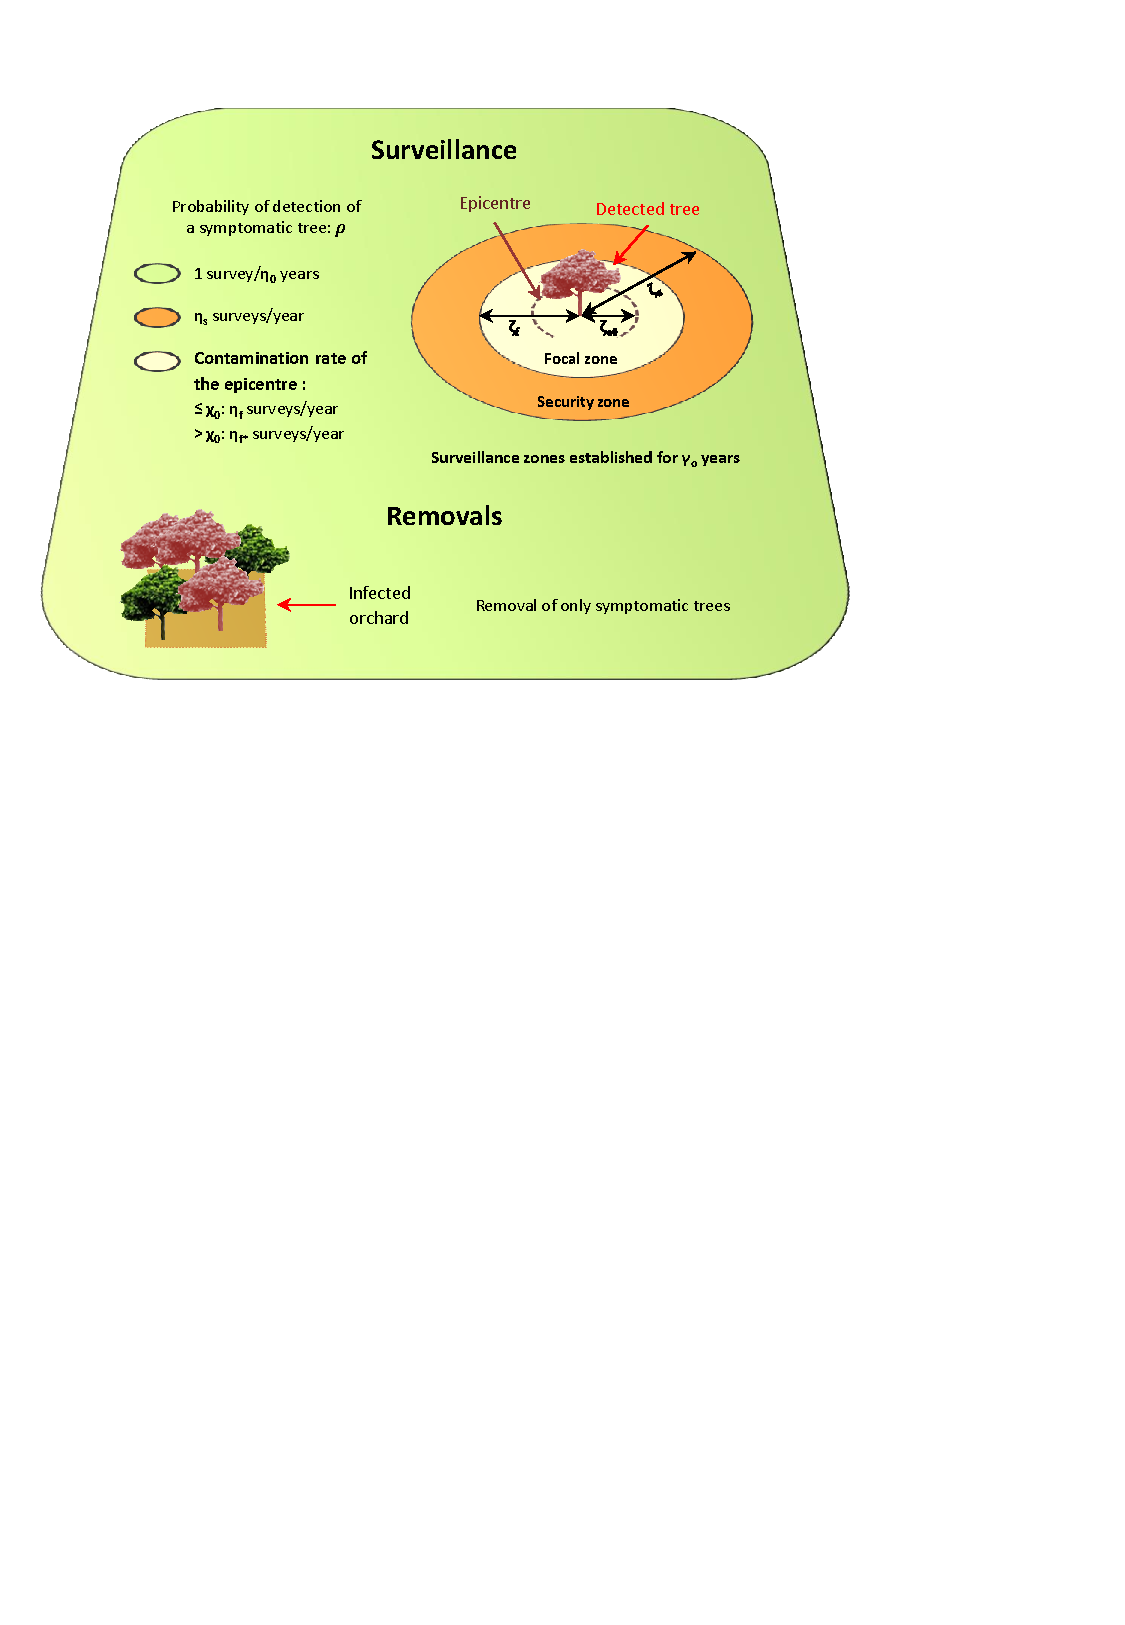
\includegraphics[trim = 0cm 16cm 4cm 1cm, clip, width=\textwidth]{Figures_Warping_paras_de_gestion.pdf}
		\caption{Management actions implemented in the model.}\label{fig:schemagestion}
	\end{figure}
	
	% Table invariances paras de gestion
	\begin{table}[htbp]
		\centering
		\caption{Invariances of management parameters. For instance, when  $\gamma_{O}$ = 0 or when $\rho$ = 0, $\chi_{o}$ does not influence the model output. }
		\begin{tabular}{|c|c|c|c|}
			\midrule
			\textbf{Management parameters} & \textbf{OR} & \textbf{OR} & \textbf{OR} \\
			\midrule
			$\rho$ & & & \\
			\midrule
			1/$\eta_{0}$ & & & \\
			\midrule
			$\gamma_{O}$ & & & \\
			\midrule
			$\chi_{o}$ & $\gamma_{O}$ = 0 & $\rho$ = 0 & \\
			\midrule
			$\zeta_{eO}$ & $\gamma_{O}$ = 0 & $\zeta_{s}$ = 0 & $\rho$ = 0\\
			\midrule
			$\zeta_{f}$ & $\gamma_{O}$ = 0 & $\zeta_{s}$ = 0 & \\
			\midrule
			$\eta_{f*}$ & $\gamma_{O}$ = 0 & $\rho$ = 0 & \\
			\midrule
			$\zeta_{s}$ & $\gamma_{O}$ = 0 & $\eta_{s}$ = 0 & \\
			\midrule
			$\eta_{s}$ & $\gamma_{O}$ = 0 & & \\
			\midrule
			$\eta_{f}$ & $\gamma_{O}$ = 0 & & \\
			\midrule
			
		\end{tabular}%
		\label{tab:table_invariances_parameters}%
	\end{table}%
	
	
	\section{Methods: Bayesian optimization}\label{sec:bo}
	
	\subsection{Overview}
	Bayesian optimization can be seen as a modernization of the statistical response surface
	methodology for sequential design~\cite{box1987empirical}, where the basic idea is to replace an expensive function by a cheap-to-evaluate surrogate one.
	In BO, Gaussian process (GP) regression, or kriging, is used to provide flexible response surface fits.
	GPs are attractive in particular for their tractability, 
	since they are simply characterized by their mean $m(.)$ and covariance (or kernel) $k(.,.)$ functions, see e.g., \citet{Rasmussen2006}. 
	In the following, we consider zero-mean processes ($m = 0$) for the sake of conciseness.
	
	Conditionally on $n$ noisy observations $\f = (f_1, \ldots, f_n)$, with independent, centered, Gaussian noise,
	that is, $f_i = y(\x_i) + \varepsilon_i$ with $\varepsilon_i \sim \mathcal{N}(0, \tau_i^2)$,
	the predictive distribution of $y$ is another GP, with mean and covariance functions given by:
	\begin{eqnarray}
	\mu(\x) & =& \textbf{k}(\x)^\top \textbf{K}^{-1} \f,  \\
	\sigma^2(\x, \x') & =& k(\x, \x') - \textbf{k}(\x)^\top \textbf{K}^{-1} \textbf{k}(\x'),
	\end{eqnarray}
	where $\textbf{k}(\x) := (k(\x, \x_1), \dots, k(\x, \x_n))^\top$ and $\textbf{K} := (k(\x_i, \x_j) + \tau_i^2 \delta_{i=j})_{1 \leq i,j \leq n}$,
	$\delta$ standing for the Kronecker function.
	
	Commonly, $k(.,.)$ belongs to a parametric family of covariance functions such as the Gaussian and Mat\'ern kernels, 
	based on hypotheses about the smoothness of $y$. Corresponding hyperparameters are often obtained as maximum likelihood estimates, 
	see e.g., \citet{Rasmussen2006} or \citet{Roustant2012} for the corresponding details.   
	
	BO typically tackles optimization problems of the form:
	\begin{eqnarray*}
		\min & y(\x) \\
		s.t. & \x \in \Xset,
	\end{eqnarray*}
	with $\Xset \in \Rset^d$ is usually a bounded hyperrectangle and $y:\Rset^d \rightarrow \Rset$ is a scalar-valued objective function.
	
	Optimization amounts here to choosing a sequence of points $\x_{n+1}, \ldots, \x_{n+N}$ at which the function $y$ is evaluated.
	Sequential design decisions, so-called {\em acquisitions}, are based on the GP model and judiciously balance exploration and exploitation 
	in search for global optima. The GP model is updated after each new value is calculated.
	
	In the noiseless setting ($\tau=0$), the canonical acquisition function is {\em expected improvement} (EI)~\cite{jones1998efficient}. 
	Define $f_{\min} = \min_{i=1,\ldots,n} y_i$, the smallest $y$-value seen so
	far, and let $I(\x) = \max\{ 0, f_{\min} - Y(x) \}$
	be the {\em improvement} at $x$.  $I(x)$ is largest when $Y(\x)$ has
	substantial distribution below $f_{\min}$. 
	The expectation of $I(x)$ over $Y(x)$ has a convenient closed form,
	revealing balance between exploitation ($\mu(x)$ under $f_{\min}$) and
	exploration (large $\sigma^{n}(x)$):
	\begin{equation}
	\esp \{I(x)\} = (f_{\min} - \mu(x)) \Phi\left(
	\frac{f_{\min} - \mu(x)}{\sigma(x)}\right)
	+ \sigma(x) \phi\left(
	\frac{f_{\min} - \mu(x)}{\sigma(x)}\right),
	\label{eq:ei}
	\end{equation}
	where $\Phi$ ($\phi$) is the standard normal cdf (pdf).
	
	\subsection{Bayesian optimization of stochastic simulators}
	When $y$ is only available through noisy evaluations, the EI acquisition cannot be used directly.
	Several authors have tackled this issue; we refer to \cite{picheny2013benchmark} for a review on the topic.
	We chose here to focus on the \textit{reinterpolation method} proposed in \cite{forrester2006design}, which is based on the use of an instrumental noiseless kriging model, 
	built from the original one. First, the (noisy) kriging predictions at the DOE points $\mu(\x_1), \ldots, \mu(\x_n)$ are computed. 
	Then, a reinterpolating model is built, by using the same covariance kernel and parameters and the same experimental design, but
	the observation vector is replaced by $\mu(\x_1), \ldots, \mu(\x_n)$ and the noise variance is set to zero. Since this latter model is
	noise-free, the classical EI can be used as the infill criterion. Once the new design is chosen and the evaluation is performed,
	both kriging models are updated. One particular characteristic of this strategy is that it does not allow repetitions, which is desirable in our
	case.
	
	\subsection{Bayesian optimization with invariances}
	
	\subsubsection{Definitions}
	\victor{to link with the problem in Section \ref{sec:model}}
	
	We can define different conditions:
	\begin{itemize}
		\item SIMPLE: if $x_i = c_i$ then $y$ is invariant w.r.t.  $\x_J$ ($J$ a subset of $\{1, \ldots, d\}$); 
		%  \item MULTIPLE: if $x_i \in \{c_{i1}, \ldots, c_{in}\}$, then $y$ is invariant w.r.t.  $\x_J$ ($J$ a subset of $\{1, \ldots, d\}$); 
		\item AND: if all $\x_I = \cc_I$ then $y$ is invariant w.r.t.  $\x_J$ (both $I$ and $J$ are subsets of $\{1, \ldots, d\}$, and $I \cap J = \emptyset$);
		\item OR: if at least one $\x_I = \cc_I$ then $y$ is invariant w.r.t.  $\x_J$ (both $I$ and $J$ are subsets of $\{1, \ldots, d\}$, and $I \cap J = \emptyset$);
		\item COMBINATION: of the above.
	\end{itemize}
	
	\subsubsection{Principle of input warping}
	\victor{to do...}
	
	\cite{snoek2014input,marmin2018warped}
	
	
	\subsubsection{Simple warping}
	\victor{Move some of this to the previous subsection}
	We first consider the case of a single invariance, $x_i = c_i$, for which a subset $\x_J$ becomes non influent. 
	In the following we use the notation $\x = (x_i, \x_J, \x_{-iJ})$ to make the $\Xset$ space decomposition explicit (note that this is only notation, 
	no actual permutation is done).
	
	A simple way to handle this problem is to distort locally the space so that the subspace $\{(x_i, \x_J) | x_i = c_i\}$ collapses to a single point,
	for instance with $\x_J$ at its average value: $(c_i, \overline{\x_J})$.
	Hence, we are seeking warping functions of the form: 
	\begin{eqnarray*}
		\psi: \Xset &\rightarrow& \widetilde{\Xset} \\
		\x & \mapsto &  \widetilde{\x}
	\end{eqnarray*}
	such that:
	\begin{enumerate}
		\item $\psi(x_i, \x_J, \x_{-iJ}) = (c_i, \overline{\x_J}, \x_{-iJ})$ if and only if $x_i=c_i$;%and $\psi(x_i, \x_J) \neq (c_i, \overline{\x_J})$ if $x_i \neq c_i$;
		\item $\psi$ restricted to $\Xset \backslash (c_i,.,.)$ and $\widetilde{\Xset} \backslash (c_i,\overline{\x_J},.)$ is a diffeomorphism;
		\item the deformation decreases monotonically when $\lvert x_i - c_i\rvert$ increases, that is: 
		\begin{eqnarray*}
			\left( \left(x_i^{k}, \x_J, \x_{-iJ} \right), \psi\left[\left(x_i^{k}, \x_J, \x_{-iJ}\right)\right] \right)\leq d \left( \left(x_i^{l}, \x_J, \x_{-iJ} \right), 
			\psi\left[\left(x_i^{l}, \x_J, \x_{-iJ}\right)\right]\right)  \\ \text{ if }\lvert x_i^{k}- c_i\rvert \leq \lvert x_i^{l}- c_i\rvert, 
		\end{eqnarray*}
		
		%   \x^{k} = (x_i^{k}, \x_J^{k}), \x^{l} = (x_i^{l}, \x_J^{l}) \text{ and } 
		%  \item the deformation tends to zero far away from the critical value:
		%  $$\lim_{\lvert x_i - c_i\rvert \rightarrow +\infty} d \left( \x, \widetilde{\x} \right) = 0$$
		for some distance $d(.,.)$.
	\end{enumerate}
	
	% We consider first here 2D functions: $y(x_1, x_2)$, and impose first invariance at $x_1=c_1$. 
	Assuming that the $\x_J$ dimension collapses to $\overline{\x_J}$ at $x_i=c_i$, we write:
	\begin{equation}
	\forall j \in J, \quad \widetilde{x_j} = \overline{x_j} + \left( x_j - \overline{x_j}\right)\alpha(x_i, c_i),
	\end{equation}
	with $\alpha(x_i, c_i)$ an attenuation function such that:
	\begin{enumerate}
		\item $\alpha(c_i, c_i) = 0$;
		\item $\alpha$ increases monotonically with $\lvert x_i - c_i\rvert$;
		\item $0 < \alpha \leq 1$, $\forall x_i \neq c_i$.
	\end{enumerate}
	Condition 1 ensures that $\widetilde{x_j} = \overline{x_j}$ when $x_i=c_i$ (the j-th dimension collapses).
	
	We propose linear and correlation-based attenuation functions: 
	\begin{eqnarray}
	\alpha_\text{lin}(x_i, c_i) &=& \frac{\lvert x_i - c_i \rvert}{\delta_i}, \\
	\alpha_\text{cor}(x_i, c_i) &=& 1 - r(x_i, c_i),
	\end{eqnarray}
	where $r$ is a $\Rset \times \Rset\rightarrow \Rset$ correlation function.
	Typically, $\delta_i$ may be set to the range of variation of $x_i$, so that the condition $\alpha \leq 1$ is ensured.
	Choosing $r$ as the generalized exponential correlation, we have:
	\begin{equation}
	\alpha_\text{exp}(x_i, c_i) = 1 - \exp \left[ - \left(\frac{\lvert x_i - c_i \rvert}{\theta_i}\right)^d \right],
	\end{equation}
	with $\theta_i$ and $d$ positive parameters to be tuned. 
	
	Figure \ref{fig:3defsimple} shows a 2D rectangular space distorted by three warpings, when the invariance is on a boundary of $x_1$.
	Figure \ref{fig:simu2Dsimple} shows (unconditional) realizations of GPs with a Gaussian kernel applied on the warped space. 
	We see that the invariance at $x_1$ maximum is ensured. The linear warping induces a strong anisotropy, while with the two other warpings,
	the process seems stationary far from the critical value.
	
	\begin{figure}[!ht]
		\centering
		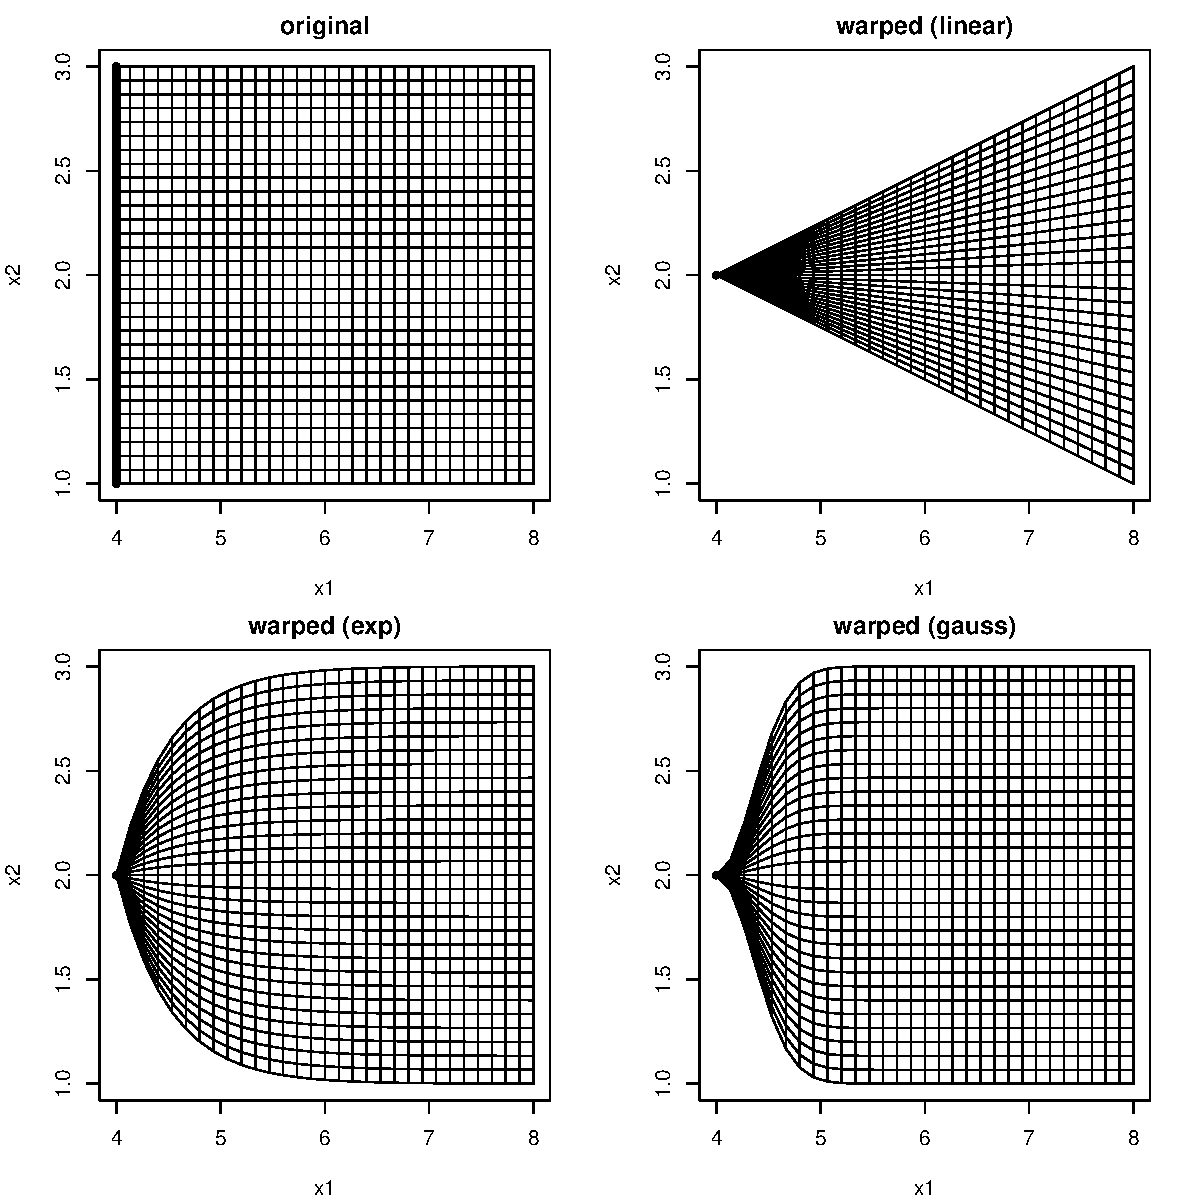
\includegraphics[width=.8\textwidth]{def2Dsimple.pdf}
		\caption{Three deformations of a 2D space. The local invariance is at $x_1=0$, highlighted with larger lines.}\label{fig:3defsimple}
	\end{figure}
	
	\begin{figure}[!ht]
		\centering
		Linear \hspace{4cm} Exp \hspace{4cm} Gauss
%%		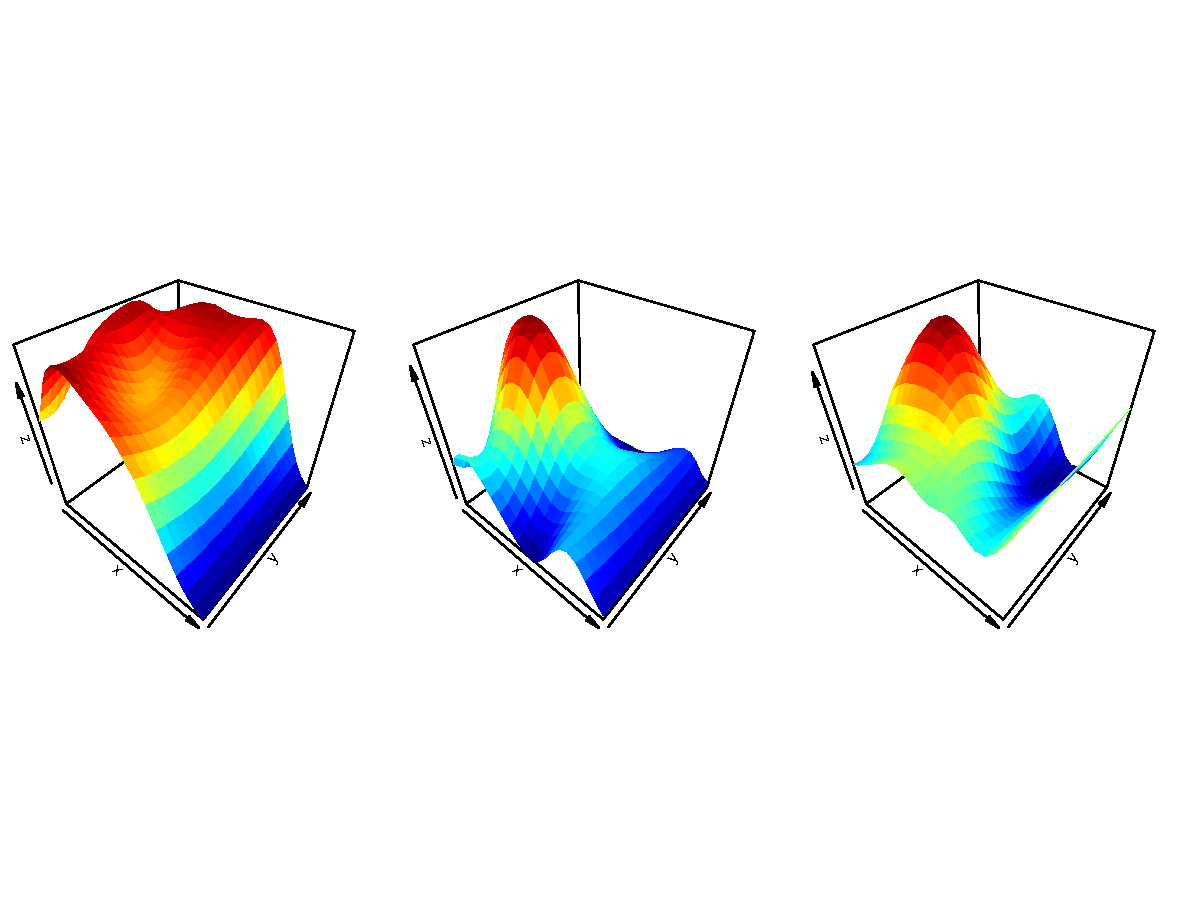
\includegraphics[trim=2mm 45mm 2mm 45mm,clip, width=\textwidth]{simu2Dsimple.pdf}
		\caption{Three GP realizations using warping functions as shown previously.}\label{fig:simu2Dsimple}
	\end{figure}
	
	\subsubsection{Warping based on linear relations}
	\victor{write everything as a linear condition and not an ``AND'' condition}
	
	Now, we consider the case where invariances occur when a set of variables takes simultaneously a set of critical values: $\x_I = \cc_I$.
	On a cubic space, this amounts to imposing invariance on an edge\footnote{such a condition 
		cannot exist in 2D under the assumption $I \cap J = \emptyset$, since $\card(J) \geq 2$.}. In that case, a possible warping is:
	\begin{equation}
	\forall j \in J, \quad \widetilde{x_j} = \overline{x_j} + \left( x_j - \overline{x_j}\right) {\alpha_I}(\x_I, \cc_I)\label{eq:and}.
	\end{equation}
	with ${\alpha_I}$ now a multivariate attenuation function ($\Rset^{\card(I)} \times \Rset^{\card(I)} \rightarrow \Rset$), so that, similarly to the simple case: 
	\begin{enumerate}
		\item $\alpha_I(\cc_I, \cc_I) = 0$;
		\item $\alpha_I$ increases monotonically with $d(\x_I, \cc_I)$ (for some distance $d(.,.)$;
		\item $0 < \alpha_I \leq 1$, $\forall \x_I \neq \cc_I$.
	\end{enumerate}
	
	As in the simple case, linear and correlation-based warpings can be defined as:
	\begin{eqnarray}
	\alpha_\text{lin}(\x_I,  \cc_I) &=& \frac{1}{\card(I)} \sum_{i \in I}\frac{\lvert x_i - c_i \rvert}{\delta_i}, \\
	\alpha_\text{cor}(\x_I,  \cc_I) &=& 1 - r_I(\x_I, \cc_I),
	\end{eqnarray}
	with $r_I$ a $\Rset^{\card(I)} \times \Rset^{\card(I)} \rightarrow \Rset$ correlation function, for instance:
	$$r_I(\x_I, \cc_I) = \exp \left[ - \sum_{i \in I}\left(\frac{\lvert x_i - c_i \rvert}{\theta_i}\right)^d \right] $$
	
	% \begin{equation}
	%  \forall j \in J, \quad \widetilde{x_j} = \overline{x_j} + \left( x_j - \overline{x_j}\right)\max_{i \in I} \alpha(x_i, c_{i}).
	% \end{equation}
	% We directly see that $\widetilde{x_j} = \overline{x_j}$ if and only if $\sum_{i \in I} \alpha(x_i, c_{i}) = 0$, which is true only for $\x_I = \cc_I$.
	% However, if we wish to ensure derivability, we need to replace the $\max$ by a smooth function. 
	
	Figure \ref{fig:def3Dedge} shows a deformation of a cubic space when $x_3$ is not influent when both $x_1$ and $x_2$ are minimal, when a Gaussian warping (exponential with $d=2$) is applied.
	\begin{figure}[!ht]
		\centering
		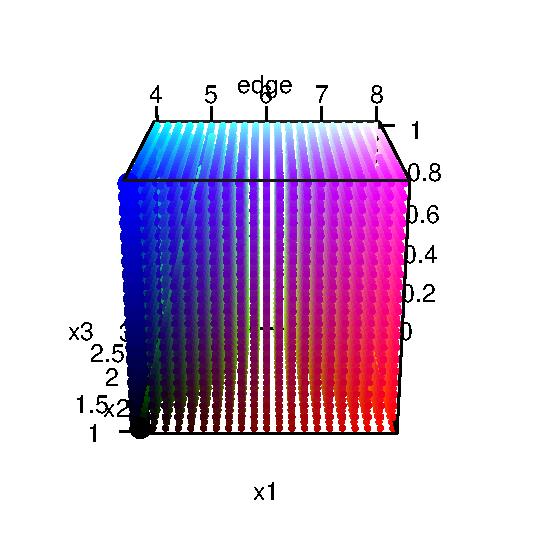
\includegraphics[width=.3\textwidth]{def3Dedge.pdf}
		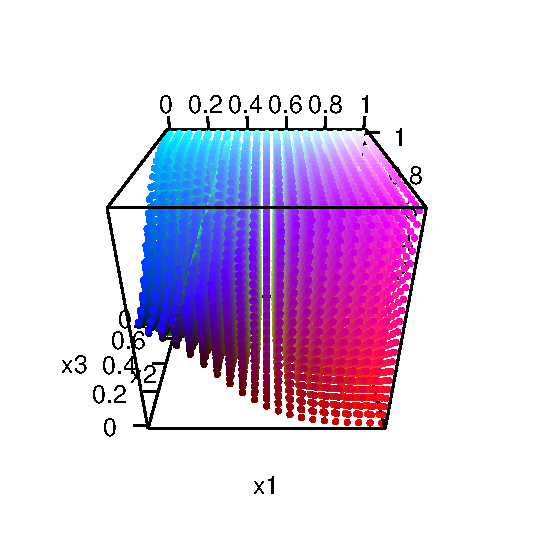
\includegraphics[width=.3\textwidth]{defAND.pdf}
		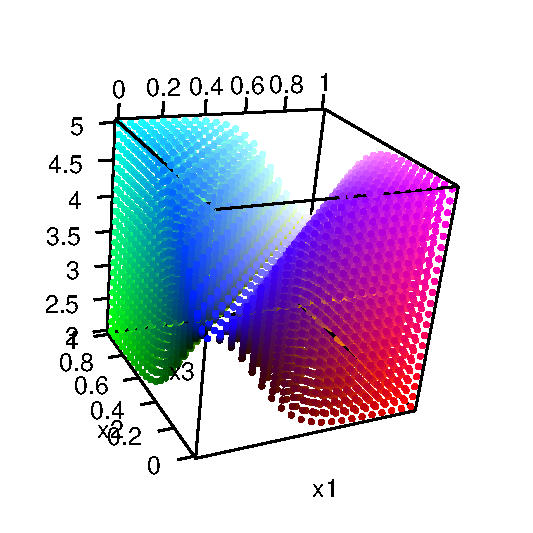
\includegraphics[width=.3\textwidth]{def3Daff.pdf}
		\caption{ Left: original space (with the critical edge highlighted). Centered: warping for $c_1=0$ AND $c_2=1$.
			Right: warping for $x_1 = x_2$.%Note that the axis has been rotated to show the shape of the distorted space.
		}\label{fig:def3Dedge}
	\end{figure}
	
	The ``AND'' condition can be generalized to the following affine formulation: 
	$y$ is invariant w.r.t. $\x_J$ if $\mathbf{A} \x_I = \mathbf{b}$, 
	with $\mathbf{A}$ a matrix of size $p \times \card(I)$ and $\mathbf{b}$ a vector of size $p$.
	For the ``AND'' condition, we have $\mathbf{A} = \mathbb{I}_p$ and $\mathbf{b}=\cc_I$.
	The warping function is the same as in Equation \ref{eq:and}, with now:
	\begin{eqnarray}
	\alpha(\x_I,  \cc_I) &=& 1 - r_A(\mathbf{A} \x_I, \mathbf{b}).\label{eq:aff}
	\end{eqnarray}
	Note that choosing the range of the correlation $r_A$ is non-trivial. A possible solution is $\theta_A = \mathbf{A}^T \boldsymbol{\theta}_I$.
	
	Figure \ref{fig:def3Dedge} (right) show the deformation of a cubic space with the condition: $y$ invariant w.r.t. $x_3$ if $x_1 = x_2$. 
	
	\subsubsection{Combining warpings}
	
	\paragraph{Independent conditions}
	Now, we consider that we have a series of invariance conditions, defined with respect to sets $I_1, \ldots, I_n$ and corresponding $J_1, \ldots, J_n$.
	% We assume that the invariance conditions are written only once for each variable, hence $J_k\cap J_l=\emptyset$, $1 \leq j\neq k \leq n$.
	If $J_k\cap J_l=\emptyset$, $1 \leq j\neq k \leq n$ and $I_i\cap J_k = \emptyset$,  $1 \leq j,k \leq n$,
	the set of warped variables are distinct from the set on which the conditions are written, 
	the invariance conditions are written only once for each variable. In that case, 
	the warpings can be applied independently.
	
	\paragraph{Combinations of simple conditions: ``OR'' invariance}
	Now, we consider the case when $y$ is invariant w.r.t. a set $\x_J$ for different conditions on sets $I_1, \ldots, I_n$
	(that, for $\x_{I_1}=\cc_{I_1}$ OR $\x_{I_2}=\cc_{I_2}$ OR $\ldots$).
	If $J\cap I_i=\emptyset$, $1 \leq i \leq n$, the warping function we propose is:
	
	\begin{equation}
	\forall j \in J, \quad \widetilde{x_j} = \overline{x_j} + \left( x_j - \overline{x_j}\right) \prod_{I \in \{I_1, \ldots, I_n \}}{\alpha_I}(\x_I, \cc_I)\label{eq:or0}. %\label{eq:orand}.
	\end{equation}
	% 
	% \begin{eqnarray}
	%  \forall j \in J, &\widetilde{x_j} =& \overline{x_j} + \left( x_j - \overline{x_j}\right) \prod_{i \in I} \alpha(x_i, c_{i})\label{eq:or0}.
	% \end{eqnarray}
	We see directly that the product of $\alpha$'s ensure that $\widetilde{x_j} = \overline{x_j}$
	if any $x_i = c_i$, and the distortion reduces only when \emph{all} the $x_i$'s are far from the $c_i$'s.
	% (instead of \emph{any} $x_i$, as in Equation \ref{eq:and}).
	% In Equation \ref{eq:or2}, it is important to notice that the $x_k$'s are centered around the $c_k$'s instead of their mean, 
	% to ensure that $\psi(\x_I, \x_J) = (\cc_I, \overline{\x_J})$ if any $x_i = c_i$.
	Figure \ref{fig:def3DORs} shows a deformation of a cubic space when $x_3$ is not influent when $x_1$ or $x_2$ are minimal, when a Gaussian warping (exponential with $d=2$) is applied.
	\begin{figure}[!ht]
		\centering
		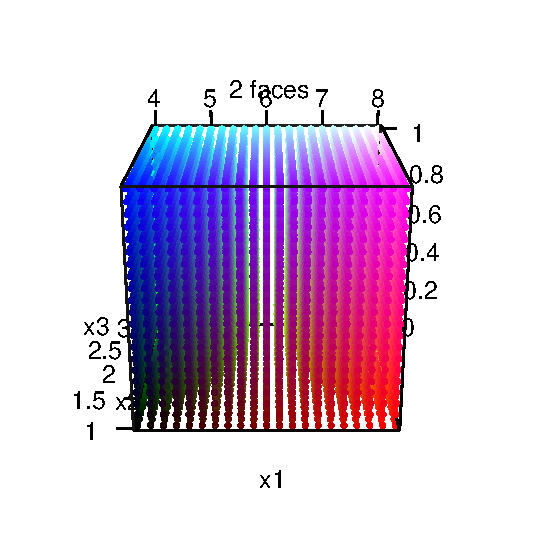
\includegraphics[width=.4\textwidth]{def3DORs.pdf}
		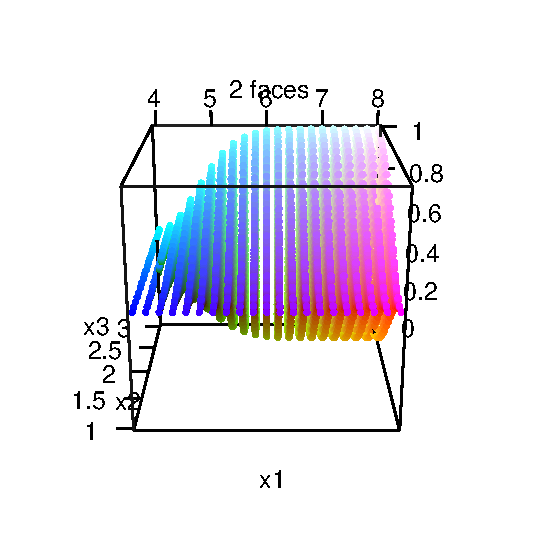
\includegraphics[width=.4\textwidth]{def3DOR2s.pdf}
		\caption{Warping for $c_1=4$ (left face of the cube) OR $c_2=1$ (front face). Left: original space, right: distorted space. %Note that the axis has been rotated to show the shape of the distorted space.
		}\label{fig:def3DORs}
	\end{figure}
	
	\paragraph{``Circular'' conditions}
	Difficulty only arises when some variables appear in both $I_l$'s and $J_m$'s sets. Take for instance a ``reciprocal'' condition, 
	e.g., $y$ is invariant w.r.t. $\x_J$ when $\x_I=\cc_I$, and invariant w.r.t. $\x_I$ when $\x_J=\cc_J$.
	In that case, applying independently warping functions would lead to: 
	\begin{eqnarray*}
		\psi(\cc_I, \x_J, \x_{-IJ}) &=& (\cc_I, \overline{\x_J}, \x_{-IJ}),\\
		\psi(\x_I, \cc_J, \x_{-IJ}) &=& (\overline{\x_I}, \cc_J, \x_{-IJ}),\\
		\text{but: } \psi(\cc_I, \cc_J, \x_{-IJ}) &=& (\cc_I, \cc_J, \x_{-IJ}),
	\end{eqnarray*}
	which induces a discontinuity.
	
	In that case, a simple solution is to fix the non influent variable to its critical value instead of its average, hence applying:
	\begin{eqnarray}
	%  \forall j \in J, &\widetilde{x_j} =& \overline{x_j} + \left( x_j - \overline{x_j}\right) \prod_{i \in I} \alpha(x_i, c_{i})\label{eq:or1},\\
	\forall k \in K= \left( \cup_{1 \leq l \leq n} I_l \right) \cap \left(\cup_{1 \leq m \leq n} J_m \right), &\widetilde{x_k} =& c_k + \left( x_k - c_k\right) \prod_{i \in I_k} \alpha(x_i, c_{i})\label{eq:or2}.
	\end{eqnarray}
	
	\paragraph{Remark} This formula does not apply in the affine case (Equation \ref{eq:aff}).
	% Unfortunately, there does not seem to be an easy solution for those cases.
	
	We first show the deformations on a 2D space on Figure \ref{fig:def2DOR}, where the two critical values are on the boundaries of $x_1$ and $x_2$.
	%, and on Figure \ref{fig:def2DT}, where one critical value is in the middle of the $x_1$ space. 
	Here, the warping of Equation \ref{eq:or2} is applied on each variable ($K=\{1,2\}$). 
	Again, except for the linear warping, the local topology is preserved far from the critical edges. 
	% On Figure \ref{fig:def2DT}, we also see that long-range distances are also unchanged.
	% A GP realization is given on Figure \ref{fig:simu2DT}. The ``T-shaped'' invariance is ensured, and the GP is stationary far from the critical values.
	
	\begin{figure}[!ht]
		\centering
		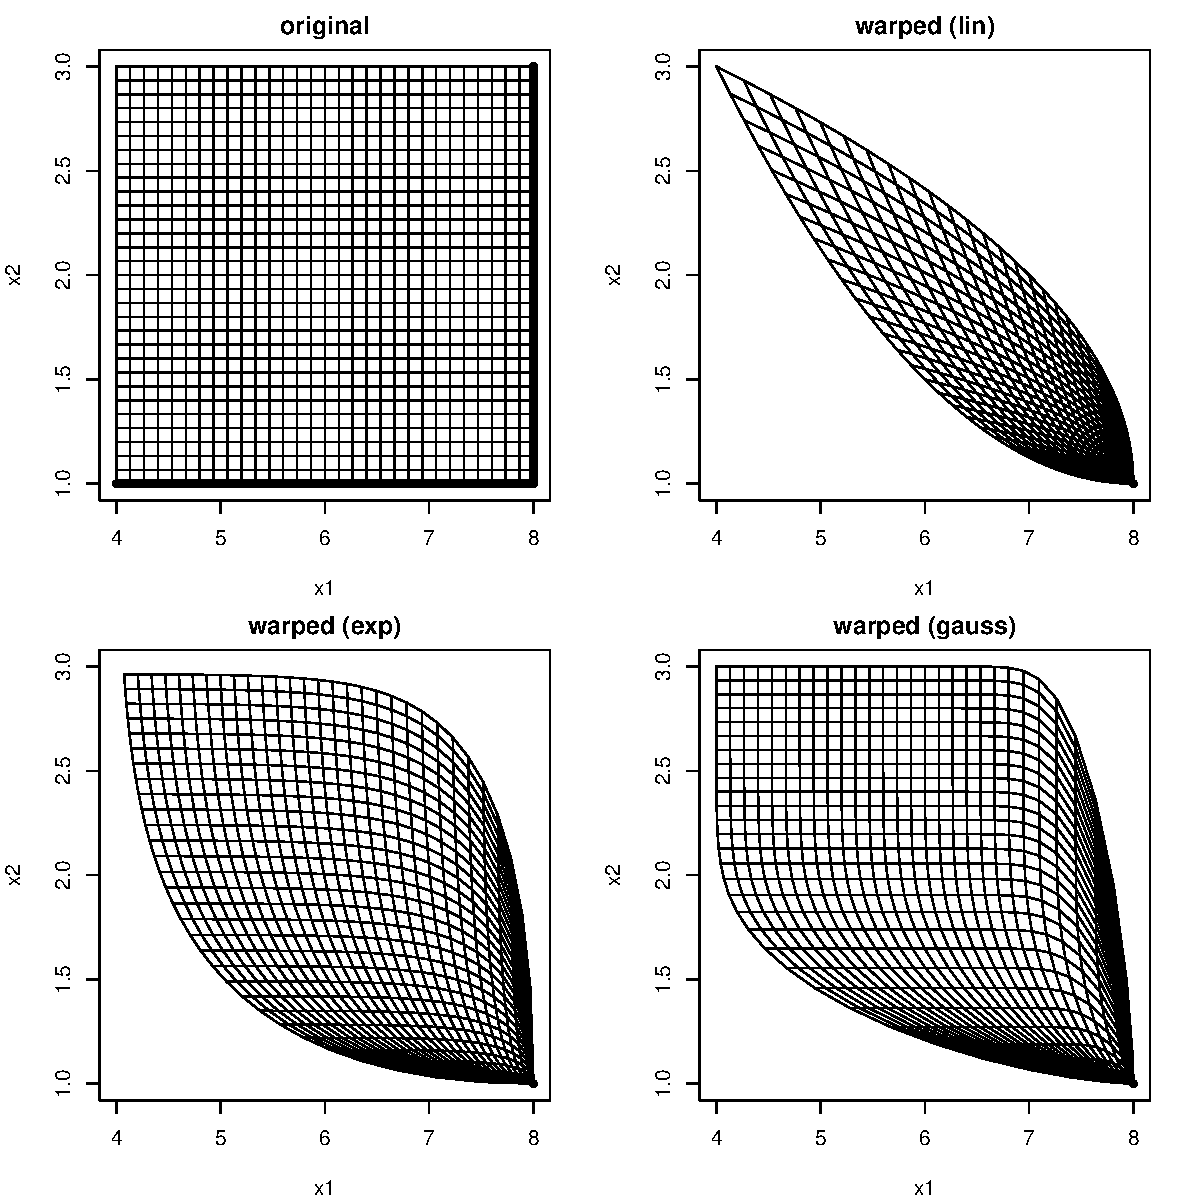
\includegraphics[width=.8\textwidth]{def2DOR.pdf}
		\caption{Three deformations of a 2D space, with invariance at $x_1=8$ OR $x_2=1$, highlighted with larger lines.}\label{fig:def2DOR}
	\end{figure}
	% 
	% \begin{figure}[!ht]
	%  \centering
	%  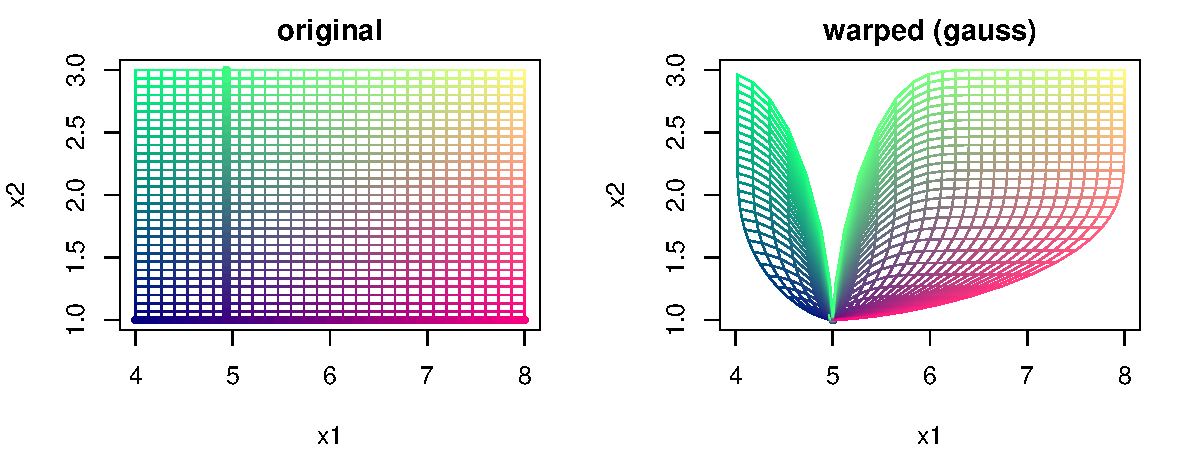
\includegraphics[width=.8\textwidth]{def2DT.pdf}
	%  \caption{Warping for a T-shaped ``OR'' invariance.}\label{fig:def2DT}
	% \end{figure}
	% 
	% \begin{figure}[!ht]
	%  \centering
	%  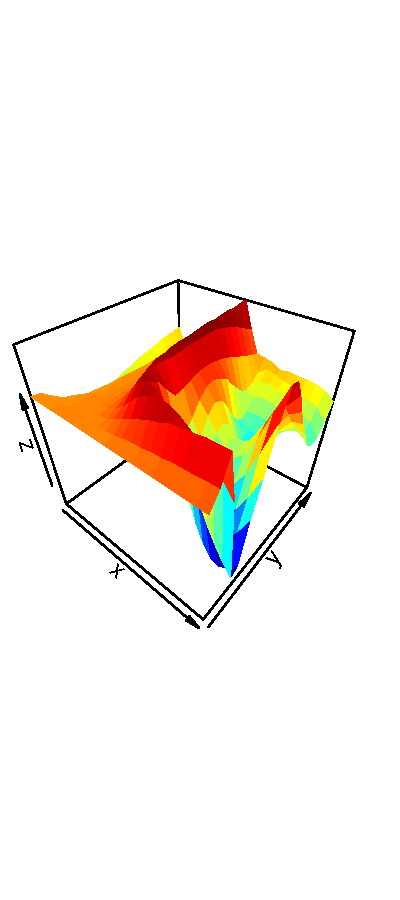
\includegraphics[trim=2mm 45mm 2mm 45mm,clip,width=.4\textwidth]{simu2DT.pdf}
	%  \caption{GP realization for a T-shaped ``OR'' invariance.}\label{fig:simu2DT}
	% \end{figure}
	
	Then, we consider a cubic space with the following circular conditions:
	\begin{itemize}
		\item $y$ is invariant w.r.t. $x_2$ if $x_1=4$;
		\item $y$ is invariant w.r.t. $x_3$ if $x_2=1$;
		\item $y$ is invariant w.r.t. $x_1$ if $x_3=0$.
	\end{itemize}
	All critical values correspond to the lower bounds of the variables.
	Equation \ref{eq:or2} is applied to each variable, hence with $K=\{1,2,3\}$, $C=[4,1,0]$ and $I_1=3$, $I_2=1$, and $I_3=2$. 
	The original and distorted space is shown in Figure \ref{fig:def3Dcirc}.
	
	\begin{figure}[!ht]
		\centering
		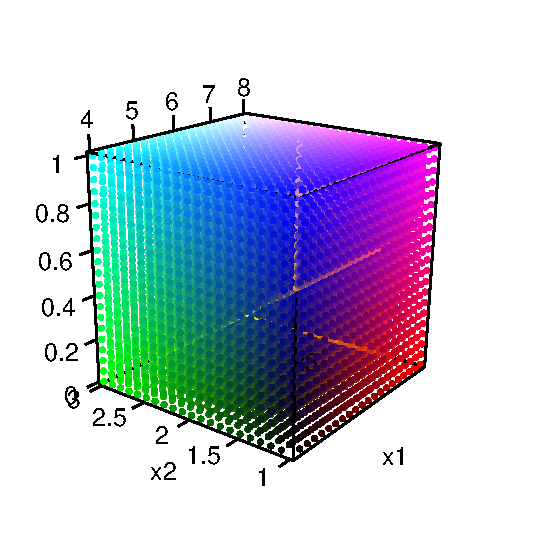
\includegraphics[width=.4\textwidth]{def3Dcirc1.pdf}
		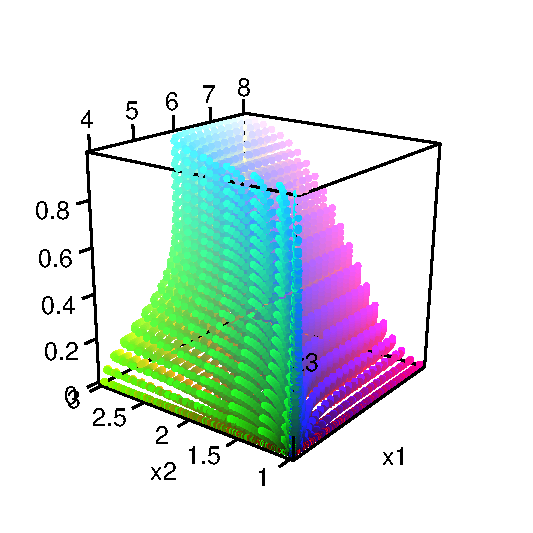
\includegraphics[width=.4\textwidth]{def3Dcirc2.pdf}
		\caption{Warping with circular conditions. Left: original space, right: distorted space.}\label{fig:def3Dcirc}
	\end{figure}
	
	% \section{Experiments on toy problems}\label{sec:exp}
	% 
	% \subsection{Problem descriptions}
	% 
	% \subsection{Comparison metrics}
	% 
	% \subsection{Results}
	
	\section{A warping-based Bayesian optimization of the Sharka model}
	
	\subsection{Numerical setup}
	
	\subsubsection{Experiments description}
	
	To evaluate the benefits of including the warping step in the optimization process (i.e. reducing the parameter space removing the combinations which lead to the same management), 
	we conducted 50 independent optimizations of sharka management parameters with and without the warping step. The criterion to optimize was the mean of the NPV ($\overline{NPV}$).
	For this to happen, we randomly selected 50 times 200 management strategies using a maximin Latin hypercube sampling design \cite{fang2005design}. 
	Then, for each sampling design of 200 strategies, we performed 2 optimizations in parallel: with and without the warping step. 
	For one optimization, we performed sequentially 200 iterations allowing to choose 200 new strategies, resulting in a total of 400 evaluated strategies.
	These 200 new strategies were selected each time among 100,000 randomly generated candidate points over the parameter space and 10,000 more locally around the best point found. 
	In addition, for each evaluated strategy, 1000 simulations were carried out (with different random seed) to take into account the variability due to the epidemic and landscape characteristics.
	
	\subsubsection{Comparison with standard BO}
	
	Description of comparison metrics
	
	\victor{Idem juste pour les méthodes de comparaison, je me charge du paragraphe pour dire à quoi on se compare et je m'occupe de la partie krigeage et warping.}
	
	\coralie{on compare ici les resultats obtenus sans le probleme d identification : avec ton script denoise.results.v6.R. Mais je ne sais pas trop comment l expliquer ici}
	
	We firstly compared the optimization results by subtracting the $\overline{NPV}$ achieved using the optimization with the warping step and the optimization without the warping step (obtained from the same sampling design). 
	
	In addition, we compared the optimization speed between the optimizations with or without warping. To this end, we used two different ways. 
	Firstly, we performed a nonlinear regression of $\overline{NPV}$ obtained for all the selected strategies during the optimization process with 
	and without the warping step, and we compared the growth parameter c of the following regression:
	$a+b \times exp^{-c\times x}$.
	
	Secondly, we used a specific algorithm developed by \coralie{reference???}. Briefly, we uniformly defined 100 $\alpha$ values between a minimum and a maximum values. 
	Then, for each iteration performed in the optimization process (i.e. for each of the 200 evaluated strategies), we add: 
	the number of optimizations (under 50) which exceed $\alpha$ 1, the number of optimizations which exceed $\alpha$ 2, ..., 
	the number of optimizations which exceed $\alpha$ 100. We used $\alpha$ $\in$ [0;18,012.12], and then $\alpha$ $\in$ [10,000;18,012.12]. 
	The value 18,012.12 corresponds to the maximal value of $\overline{NPV}$ identified in all the optimizations.
	
	\subsection{Results and insights into the Sharka model}
	
	We firstly subtracting the $\overline{NPV}$ obtained with optimizations with and without the warping step. 
	In 24 out of the 50 optimization cases, we obtained better $\overline{NPV}$ with the warping step than without (Fig.\ref{fig:waping_moins_sanswarping}). 
	This result means that with 200 iterations in the optimization, the final optimization result is not impacted by the use of a warping step.
	
	\begin{figure}[!ht]
		\centering
		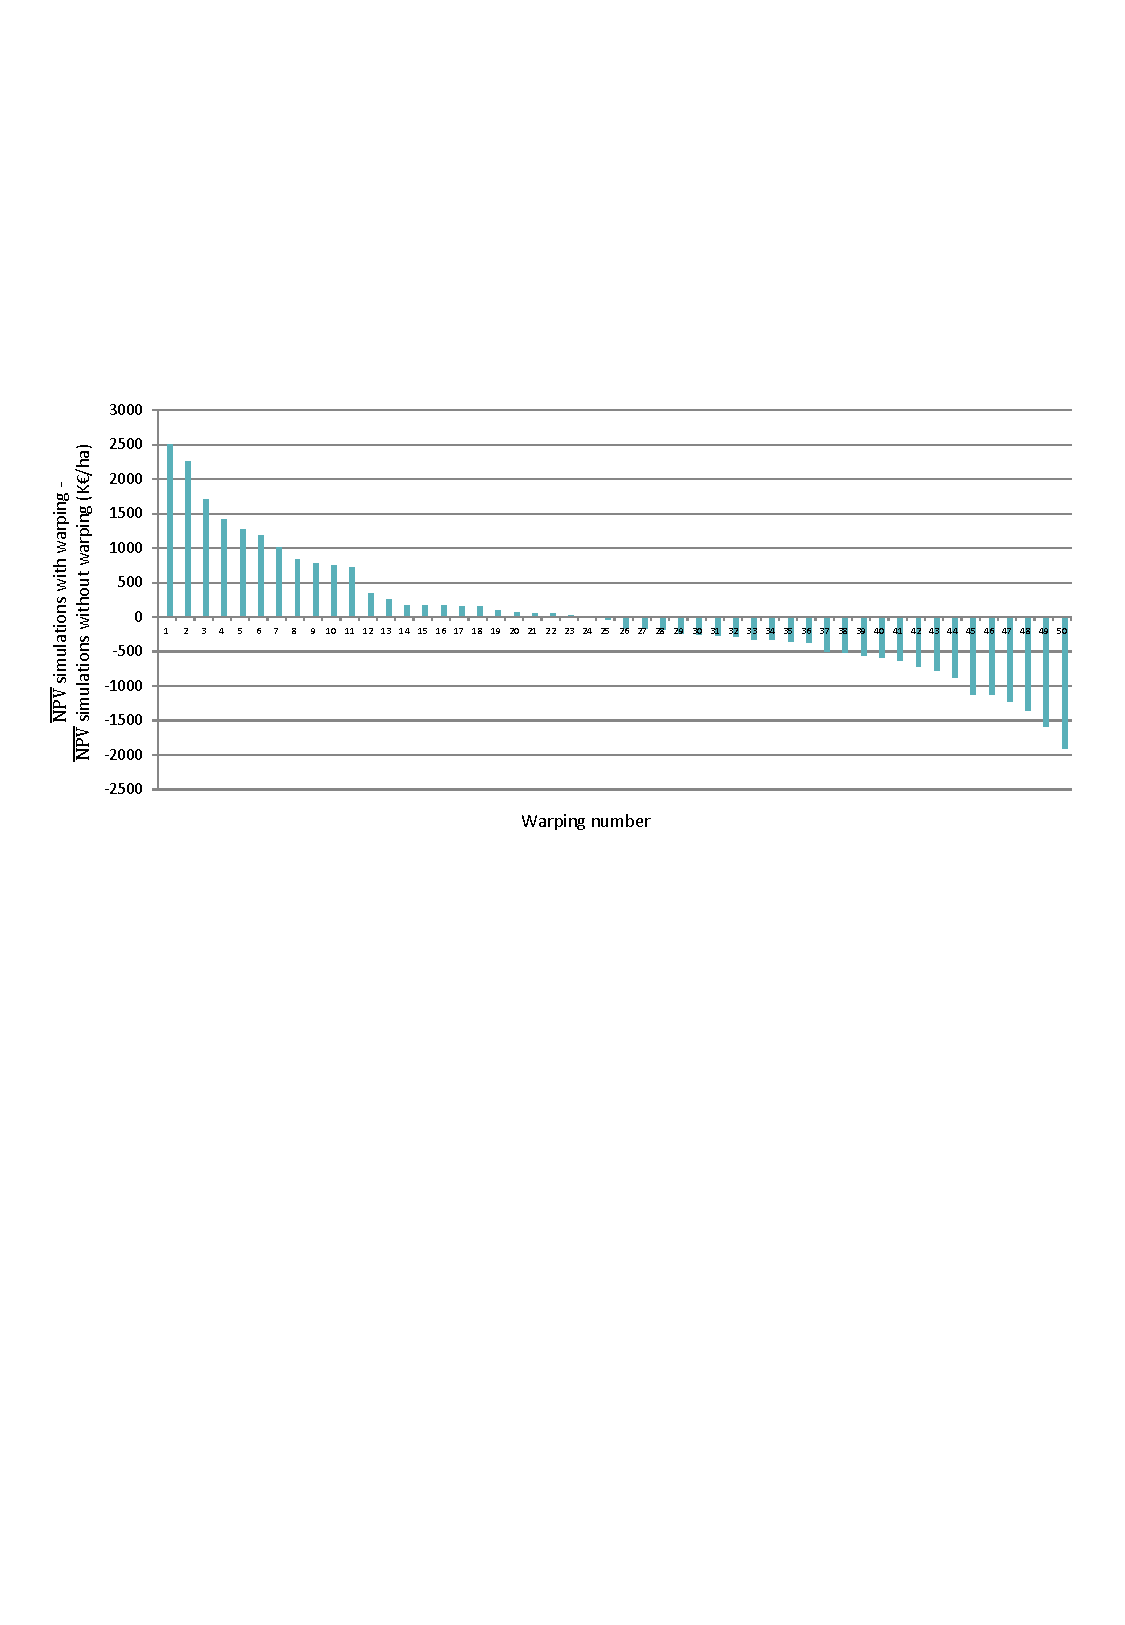
\includegraphics[trim = 2.6cm 13.5cm 3.1cm 6.8cm, clip, width=\textwidth]{Figures_Warping_resultats_warping_moins_sanswarping.pdf}
		\caption{Comparison of $\overline{NPV}$ obtained at the end of the optimization with and without warping. }\label{fig:waping_moins_sanswarping}
	\end{figure}
	
	However, we showed that the warping can impact the optimization speed (Fig.\ref{fig:moyennesNPV}). 
	Indeed, the parameter c corresponding to the growth parameter of a nonlinear regression was higher with (0.26) than without (0.18) warping (Fig.\ref{fig:nonlinear_regression}). 
	In addition, we can visually observe that the warping step allow to improve the optimization speed on the Fig.\ref{fig:algococo0} and \ref{fig:algococo10000} 
	which present the results of the algorithm developped by \coralie{reference???}.
	
	\begin{figure}[!ht]
		\centering
		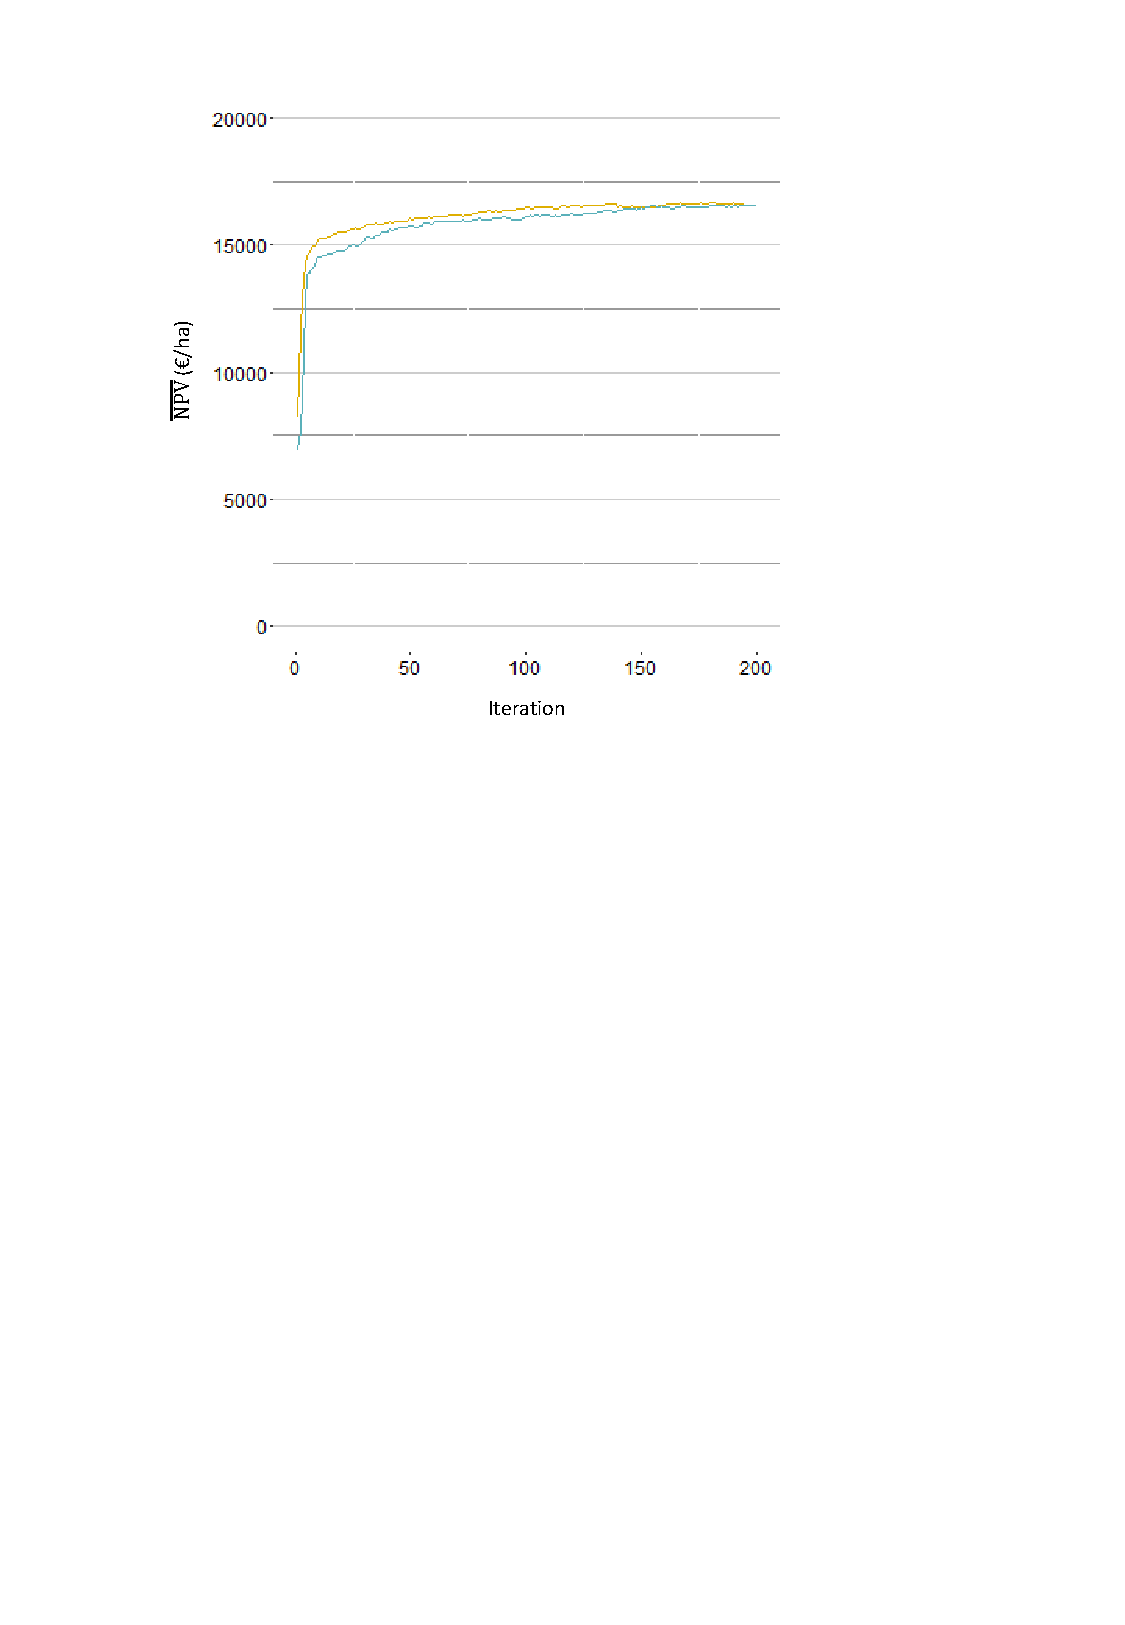
\includegraphics[trim = 3.1cm 18.1cm 2.7cm 1.9cm, clip, width=\textwidth]{Figures_Warping_resultats_courbes_moyennes_mean_NPV_warping_sanswarping.pdf}
		\caption{Comparison of $\overline{NPV}$ obtained during optimizations with and without warping. 
			Yellow and blue lines represent the mean of the $\overline{NPV}$ selected at each iteration for the 50 optimizations respectively perfomed with and without the warping step. }\label{fig:moyennesNPV}
	\end{figure}
	
	\begin{figure}[!ht]
		\centering
		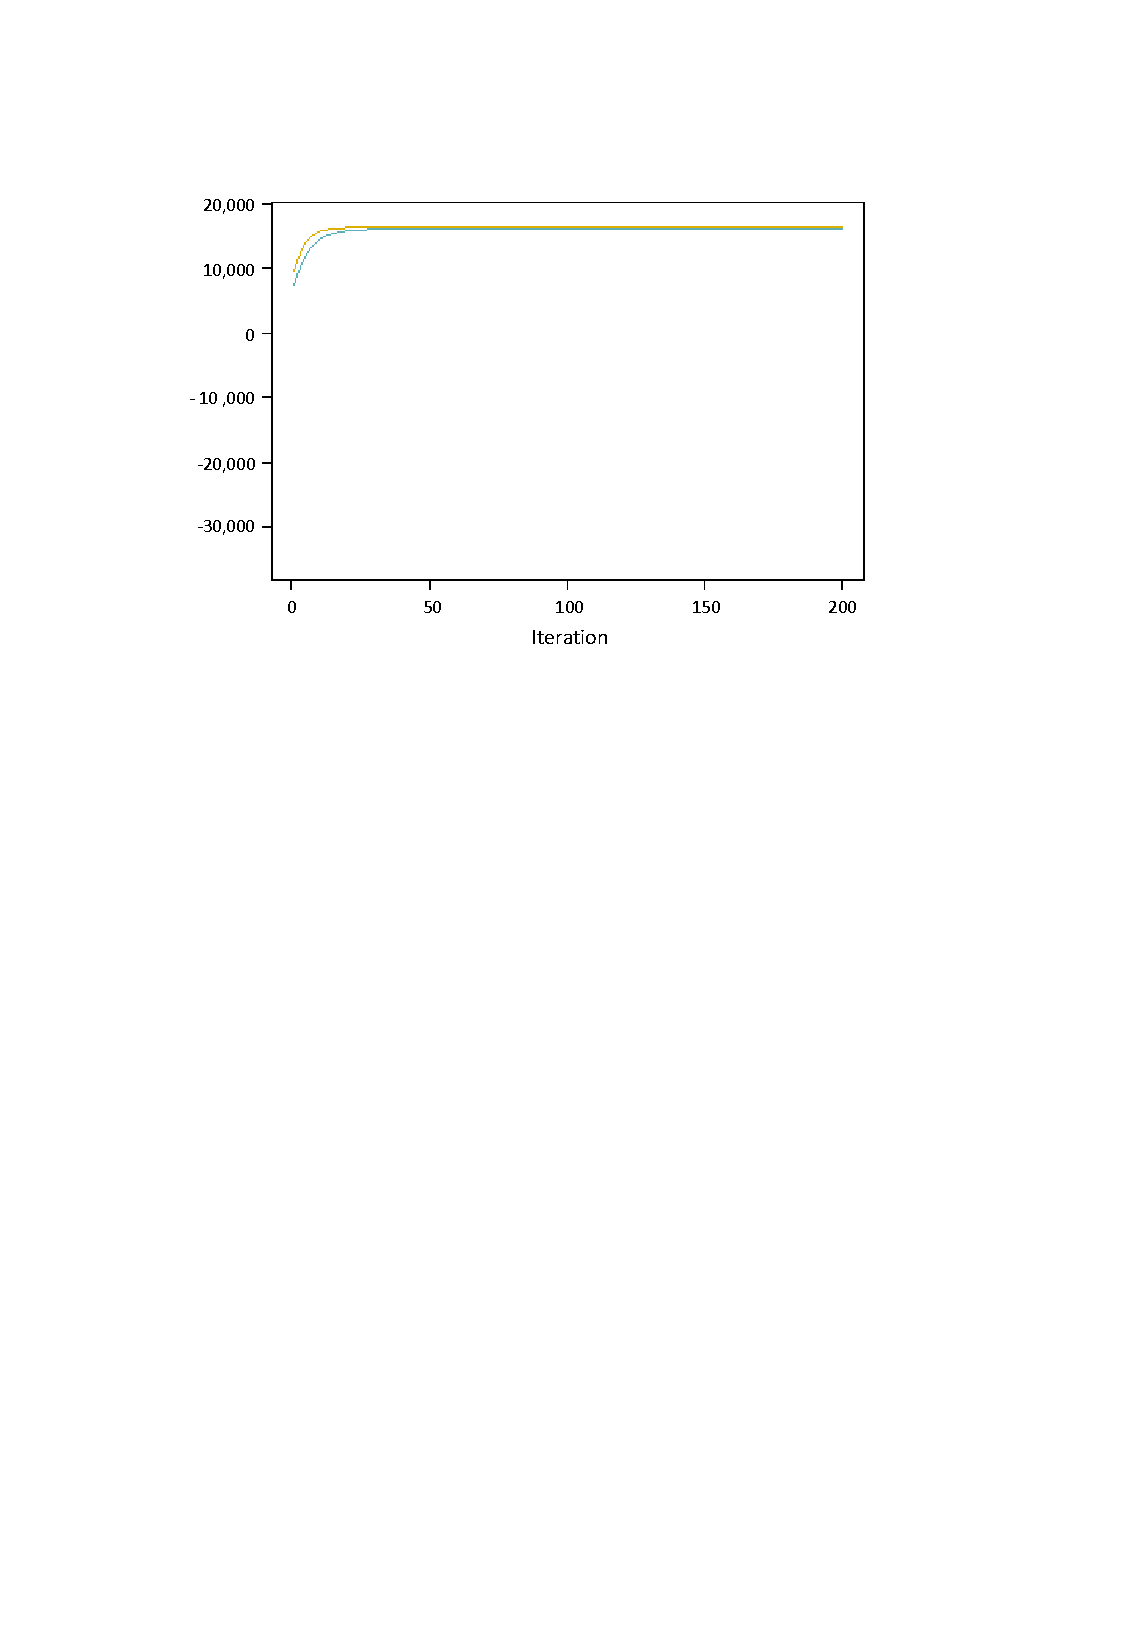
\includegraphics[trim = 3.1cm 16.4cm 4.3cm 3.3cm, clip, width=\textwidth]{Figures_Warping_resultats_courbes_regression_lineaire_warping_sanswarping.pdf}
		\caption{Non linear regression on $\overline{NPV}$ obtained at each iteration of the optimizations with (yellow) and without (blue) warping.}\label{fig:nonlinear_regression}
	\end{figure}
	
	\begin{figure}[!ht]
		\centering
		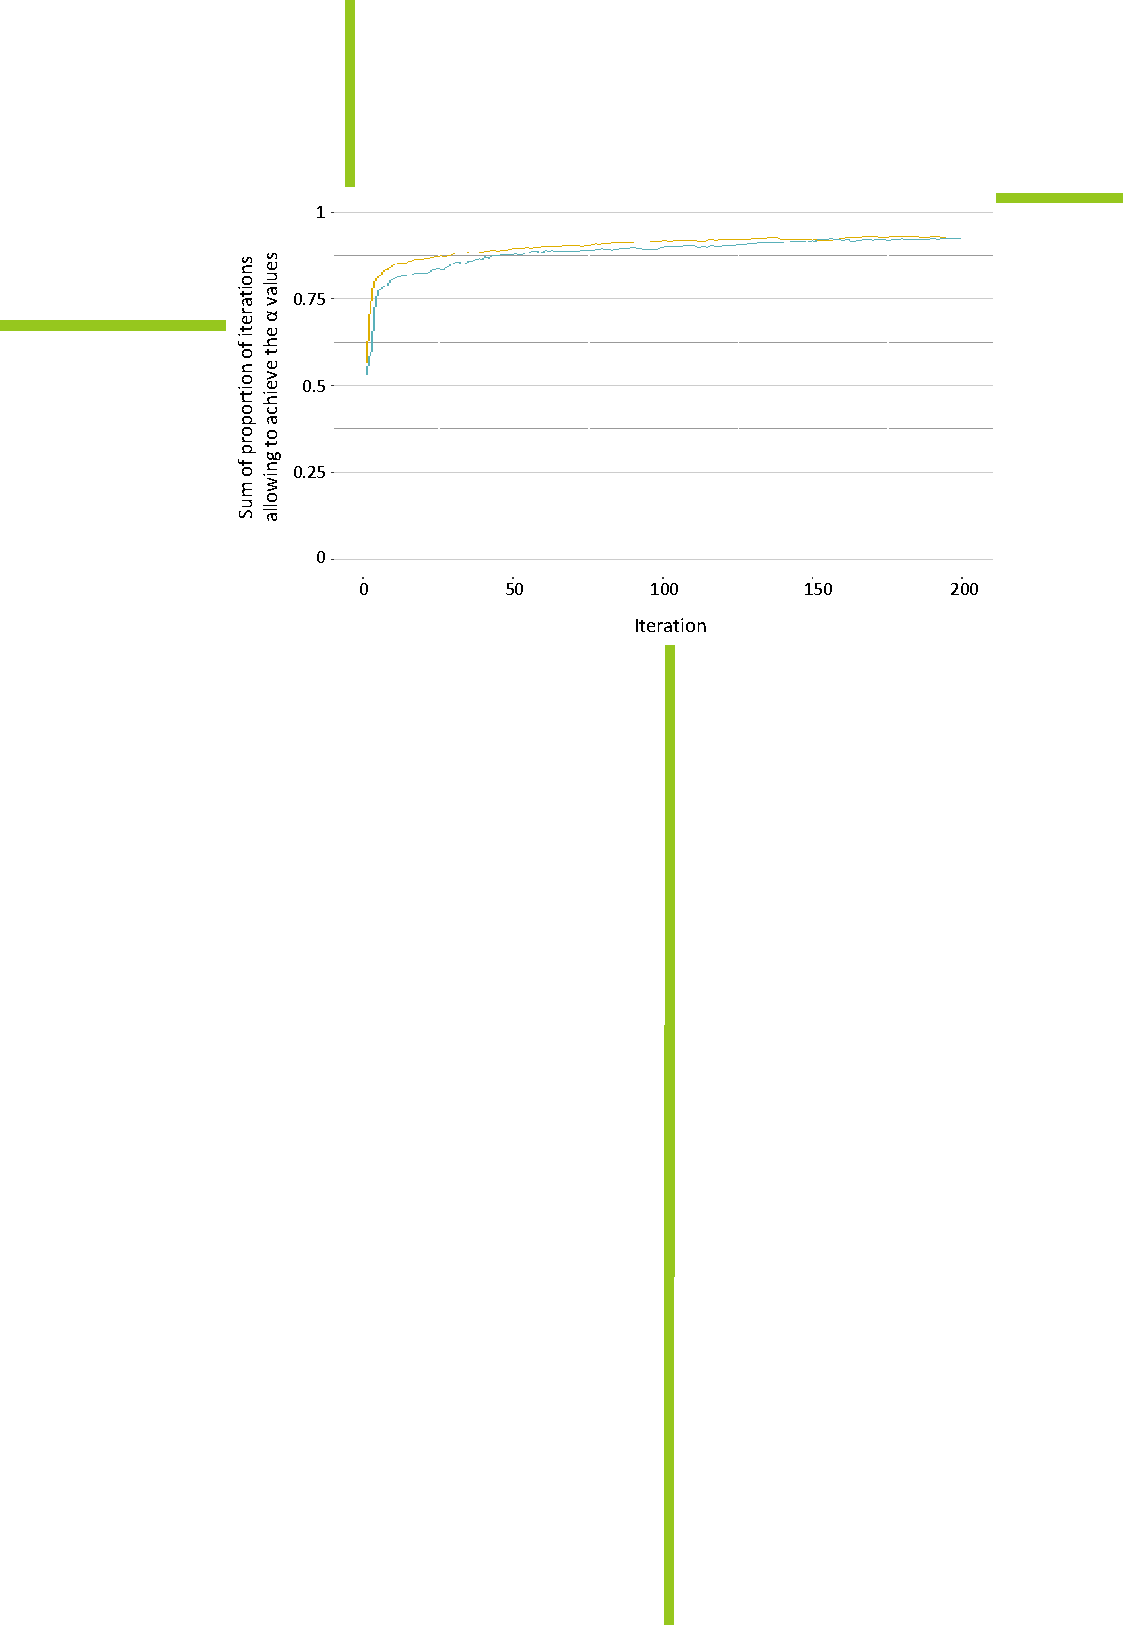
\includegraphics[trim = 4cm 16.6cm 2.2cm 3.5cm, clip, width=\textwidth]{Figures_Warping_resultats_courbes_algoCoco_0_18000.pdf}
		\caption{Results of the Coco algorithm with (yellow) and without (blue) warping ($\alpha$ $\in$ [0;18,012.12]).}\label{fig:algococo0}
	\end{figure}
	
	\begin{figure}[!ht]
		\centering
		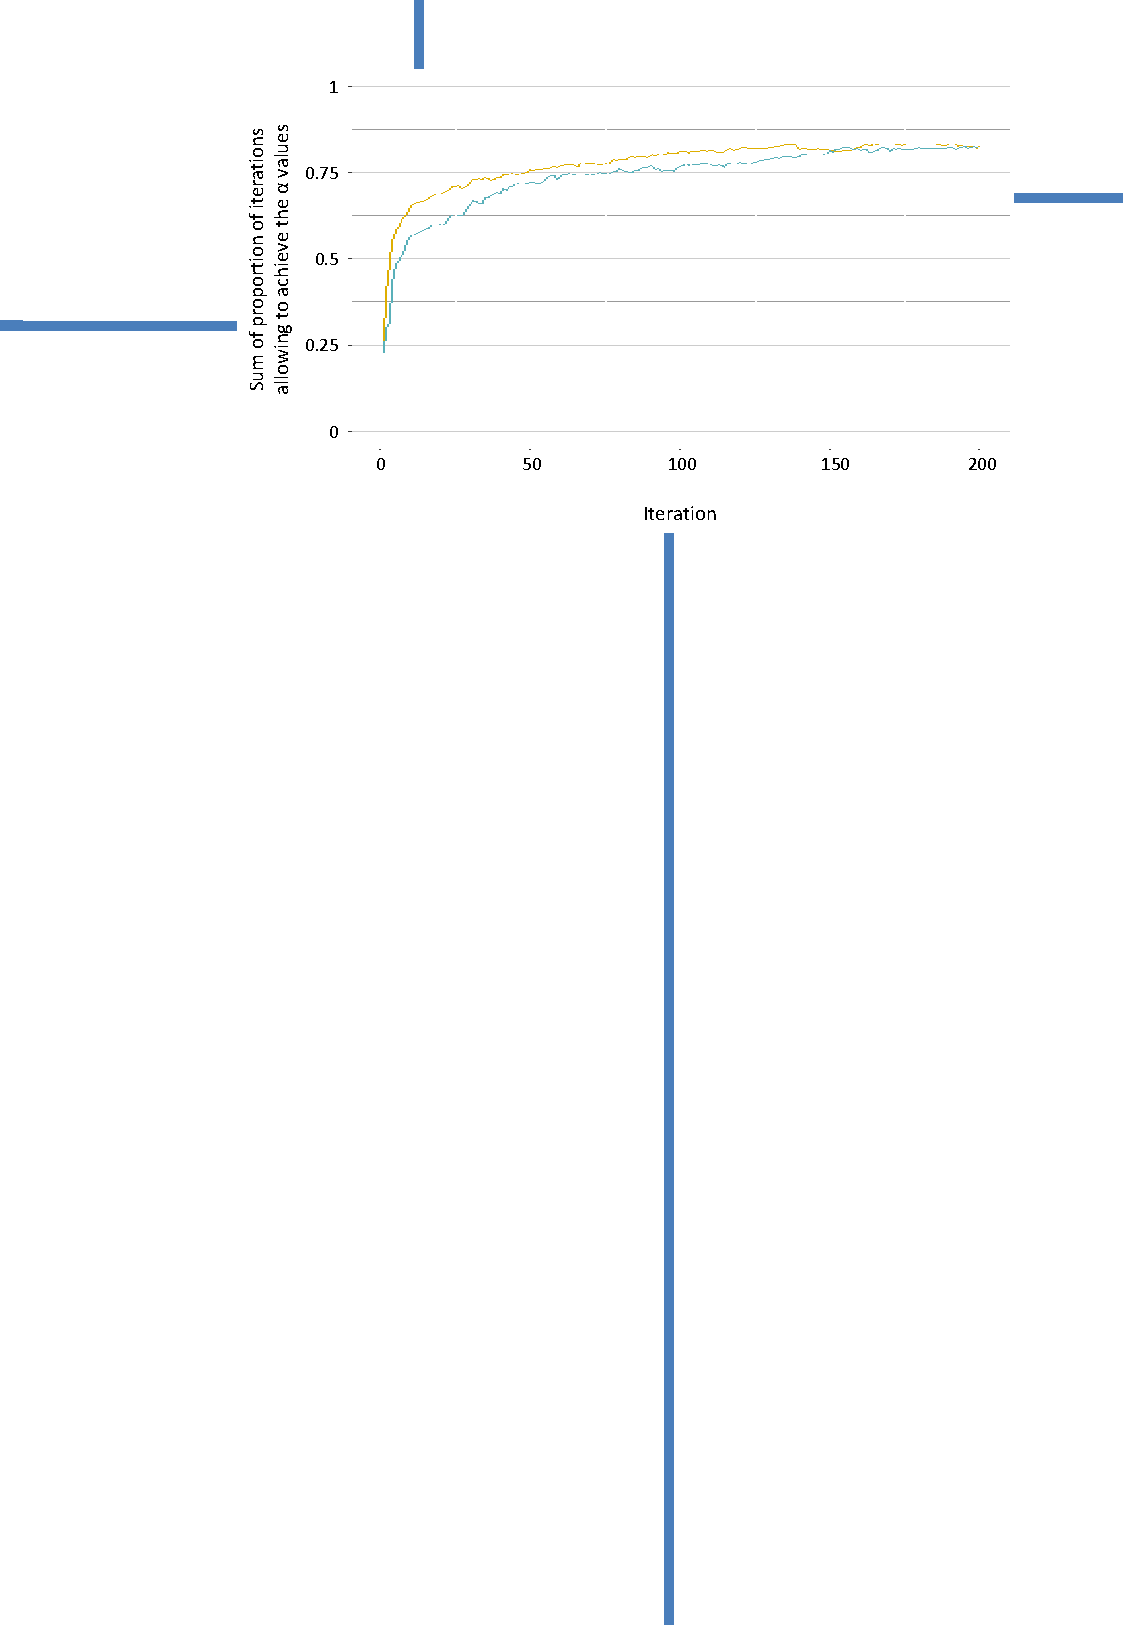
\includegraphics[trim = 4cm 18.5cm 1.9cm 1.4cm, clip, width=\textwidth]{Figures_Warping_resultats_courbes_algoCoco_10000_18000.pdf}
		\caption{Results of the Coco algorithm with (yellow) and without (blue) warping ($\alpha$ $\in$ [10,000;18,012.12]).}\label{fig:algococo10000}
	\end{figure}
	
	\section{Conclusion}
	
	What we did (the problem we solved)
	
	What we proposed: warping to tackle invariances. Proof of concept
	
	Possible extensions
	
	\section*{References}
	\bibliographystyle{spbasic}
	\bibliography{refs}
\end{document}